% Compile with XeLaTeX on Overleaf.
\documentclass[11pt,a4paper]{article}

\usepackage[UTF8]{ctex}
\usepackage[a4paper,margin=1in]{geometry}
\usepackage{graphicx}
\usepackage{booktabs}
\usepackage{float}
\usepackage{hyperref}
\usepackage{amsmath}
\usepackage{array}
\usepackage{xcolor}

\hypersetup{
    colorlinks=true,
    linkcolor=blue,
    urlcolor=blue,
    citecolor=blue
}

\newcommand{\githuburl}{\url{https://github.com/highevolutionary/Project-2-of-Neural-Network-and-Deep-Learning.git}}

\title{Project-2 of ``Neural Network and Deep Learning''}
\author{李星 \\ Student ID: 22300290002}
\date{\today}

\begin{document}
\maketitle

\begin{abstract}
This report presents the implementation and experimental analysis for Project 2.
The experiments are conducted on CIFAR-10 with VGG-A and VGG-A with Batch
Normalization. I compare classification performance, model size, training
behavior, loss landscape, and several optimization choices including filter
width, loss regularization, activation functions, and optimizers. The code,
training scripts, and trained weights are included in the GitHub repository:
\githuburl.
\end{abstract}

\section{Train a Network on CIFAR-10}

\subsection{Dataset and Experimental Setup}

CIFAR-10 contains 60,000 RGB images of size $32\times32$ from 10 classes. I used
the standard training split with 50,000 images and the test split with 10,000
images for evaluation. Images were converted to tensors and normalized with mean
$(0.5,0.5,0.5)$ and standard deviation $(0.5,0.5,0.5)$.

The main experiments were run on an NVIDIA A100-SXM4-80GB GPU. The batch size
was 128, and each main VGG experiment was trained for 20 epochs. The loss
function was cross entropy. Adam with weight decay $5\times10^{-4}$ was used for
the main comparison. The tested learning rates were
\[
    10^{-3},\; 2\times 10^{-3},\; 10^{-4},\; 5\times 10^{-4}.
\]

The GitHub repository contains all code files and trained model weights:
\githuburl. The CIFAR-10 dataset used in the experiment is the Python version of
CIFAR-10 and is also included with the submitted project files.

\subsection{Network Components}

The implemented networks contain all required components:

\begin{itemize}
    \item Fully connected layers: the classifier uses linear layers.
    \item 2D convolutional layers: feature extraction is based on \texttt{Conv2d}.
    \item 2D pooling layers: each VGG stage uses \texttt{MaxPool2d}.
    \item Activations: ReLU is used in the baseline, and LeakyReLU/ELU are used
    in ablation experiments.
\end{itemize}

For the additional component, I implemented Batch Normalization. The VGG-A-BN
model inserts \texttt{BatchNorm2d} after each convolution and before the
activation.

\subsection{Network Structures}

The baseline VGG-A follows the provided project code and is adapted to CIFAR-10.
It has five convolutional stages and a three-layer classifier. The BN version
keeps the same convolutional and classifier widths, but adds BatchNorm layers
after all convolutional layers.

\begin{table}[H]
\centering
\caption{Main model configurations.}
\begin{tabular}{lrrr}
\toprule
Model & Parameters & Best Val. Acc. & Best Error \\
\midrule
VGG-A, lr=$10^{-3}$ & 9,750,922 & 76.70\% & 23.30\% \\
VGG-A, lr=$2\times10^{-3}$ & 9,750,922 & 10.00\% & 90.00\% \\
VGG-A, lr=$10^{-4}$ & 9,750,922 & 76.83\% & 23.17\% \\
VGG-A, lr=$5\times10^{-4}$ & 9,750,922 & 79.36\% & 20.64\% \\
VGG-A-BN, lr=$10^{-3}$ & 9,756,426 & \textbf{82.17\%} & \textbf{17.83\%} \\
VGG-A-BN, lr=$2\times10^{-3}$ & 9,756,426 & 81.19\% & 18.81\% \\
VGG-A-BN, lr=$10^{-4}$ & 9,756,426 & 75.03\% & 24.97\% \\
VGG-A-BN, lr=$5\times10^{-4}$ & 9,756,426 & 81.76\% & 18.24\% \\
\bottomrule
\end{tabular}
\end{table}

The best overall model is VGG-A-BN with learning rate $10^{-3}$, achieving
82.17\% validation accuracy. The best baseline VGG-A result is 79.36\%, obtained
with learning rate $5\times10^{-4}$. The BN model improves the best error from
20.64\% to 17.83\%, while adding only 5,504 parameters.

\subsection{Optimization Attempts}

To satisfy the optimization requirements, I tested different filter widths,
regularization/loss settings, activation functions, and optimizers. These
ablation experiments were trained for 5 epochs to compare short-term convergence
under the same setting.

\begin{table}[H]
\centering
\caption{Ablation experiments for optimization choices.}
\small
\begin{tabular}{llrr}
\toprule
Experiment & Category & Parameters & Best Val. Acc. \\
\midrule
Width multiplier 0.5 & Different filters & 2,708,362 & 77.16\% \\
Width multiplier 1.0 & Different filters & 9,756,426 & 77.19\% \\
LeakyReLU & Different activations & 9,756,426 & 75.79\% \\
ELU & Different activations & 9,756,426 & 72.67\% \\
No weight decay & Loss/regularization & 9,756,426 & \textbf{78.75\%} \\
Label smoothing 0.1 & Loss/regularization & 9,756,426 & 77.45\% \\
SGD with momentum & Different optimizer & 9,756,426 & 75.98\% \\
\bottomrule
\end{tabular}
\end{table}

The short ablation shows that the smaller width multiplier significantly reduces
parameters while keeping similar early accuracy. In the 5-epoch setting, removing
weight decay gave the highest short-run validation accuracy, although this does
not necessarily imply better long-run generalization. ReLU was stronger than
LeakyReLU and ELU in this setting. Adam converged faster than SGD momentum under
the chosen hyperparameters.

\subsection{Training Curves}

\begin{figure}[H]
\centering
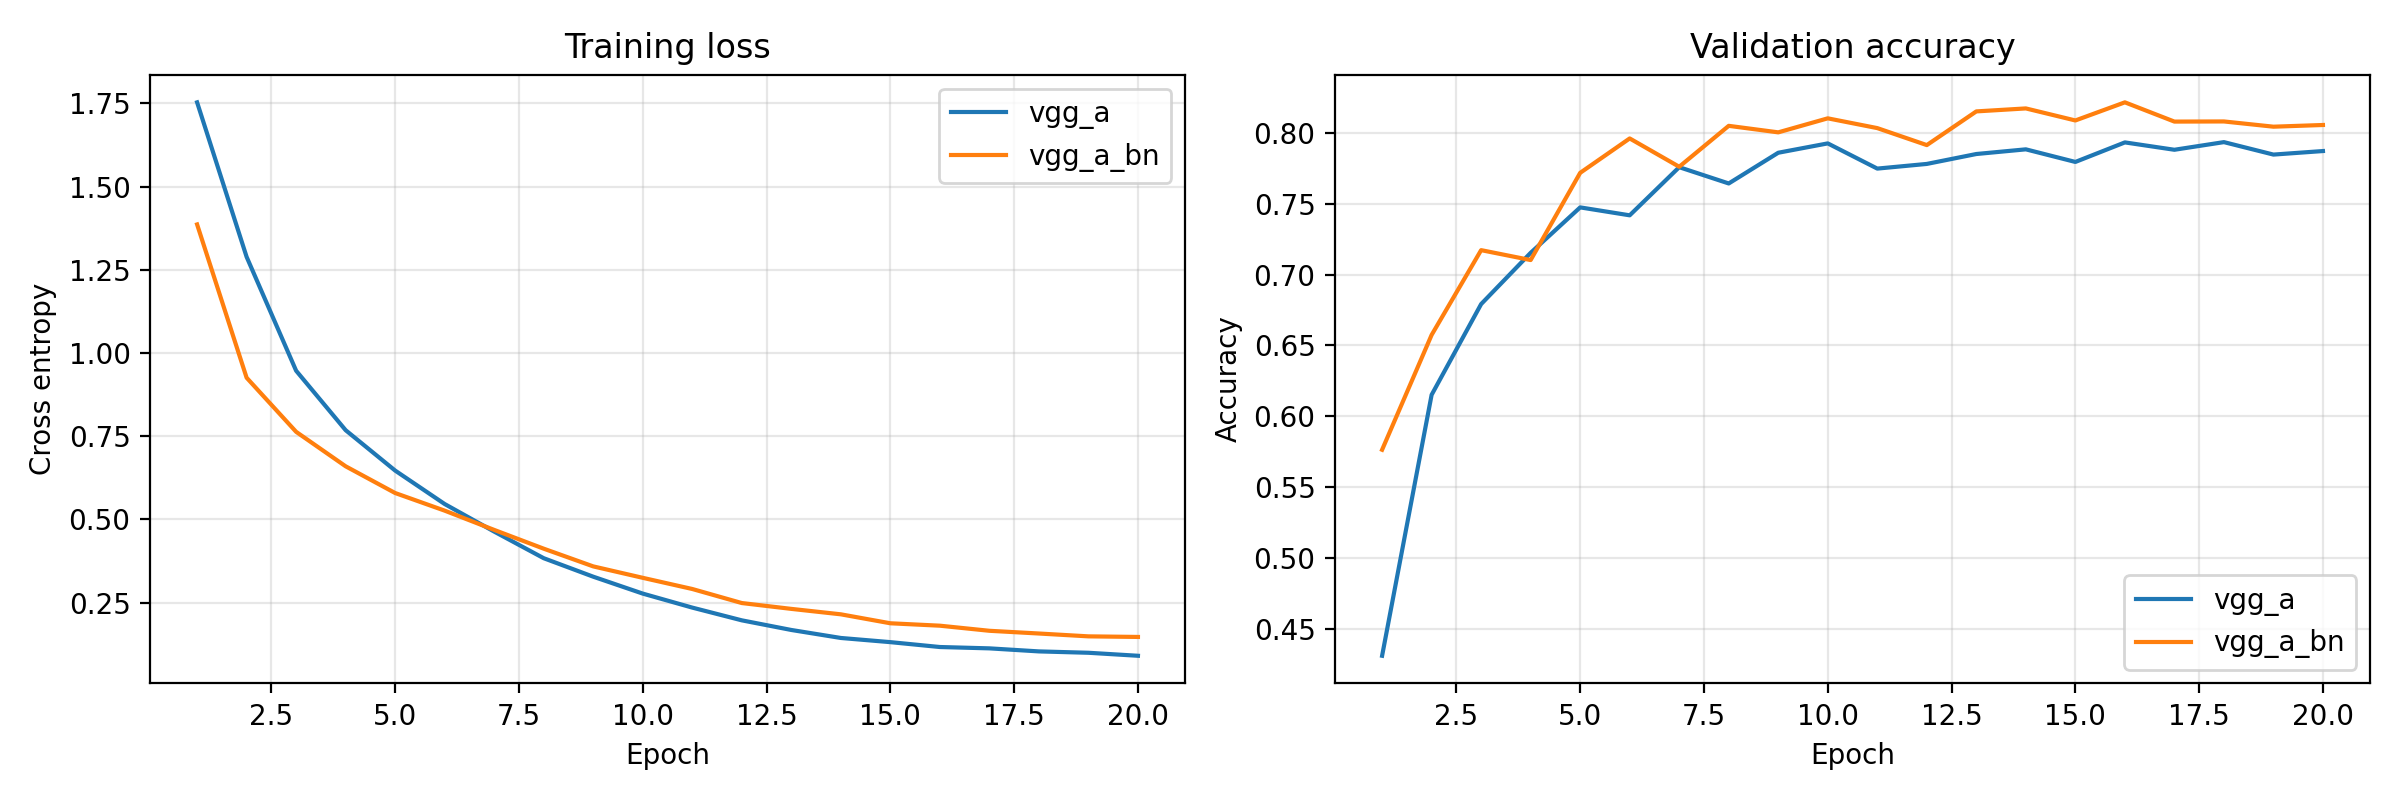
\includegraphics[width=0.95\linewidth]{figures/training_curves.png}
\caption{Training loss and validation accuracy curves for the best VGG-A and
VGG-A-BN runs.}
\end{figure}

The training curves show that both networks learn meaningful CIFAR-10 features.
The BN model reaches a higher final validation accuracy and is less sensitive to
larger learning rates. In particular, VGG-A with learning rate $2\times10^{-3}$
collapses to about 10\% accuracy, while VGG-A-BN still trains successfully with
the same learning rate. This supports the claim that Batch Normalization improves
optimization stability.

\section{Batch Normalization}

\subsection{Batch Normalization Algorithm}

For a convolutional activation tensor $I_{b,c,x,y}$, Batch Normalization
normalizes each channel using statistics computed over the mini-batch and
spatial locations:
\[
O_{b,c,x,y}
=
\gamma_c
\frac{I_{b,c,x,y}-\mu_c}{\sqrt{\sigma_c^2+\epsilon}}
+ \beta_c .
\]
Here $\mu_c$ and $\sigma_c^2$ are the channel-wise mean and variance, and
$\gamma_c,\beta_c$ are learnable affine parameters. During evaluation, running
statistics collected during training are used. In my implementation, BN layers
are inserted after convolution and before activation.

\subsection{VGG-A With and Without BN}

I compared VGG-A and VGG-A-BN under the same training protocol and learning-rate
list. The BN version performs better in the best setting and is more robust to a
large learning rate. The parameter increase is small because BN adds only
channel-wise scale and shift parameters. Therefore, the improvement is mainly due
to optimization behavior rather than a much larger model.

\section{How Batch Normalization Helps Optimization}

\subsection{Loss Landscape}

Following the provided \texttt{VGG\_Loss\_Landscape.py} idea, I trained each
model with four learning rates:
\[
[10^{-3},\;2\times10^{-3},\;10^{-4},\;5\times10^{-4}].
\]
For each training step, the loss values from all learning-rate runs were aligned.
Then I computed
\[
\text{min\_curve}_t = \min_i L_{i,t}, \qquad
\text{max\_curve}_t = \max_i L_{i,t},
\]
where $L_{i,t}$ is the loss at step $t$ for learning-rate run $i$. I plotted both
curves and filled the region between them using
\texttt{matplotlib.pyplot.fill\_between}. The same procedure was applied to
VGG-A and VGG-A-BN, and both results are shown in one figure.

\begin{figure}[H]
\centering
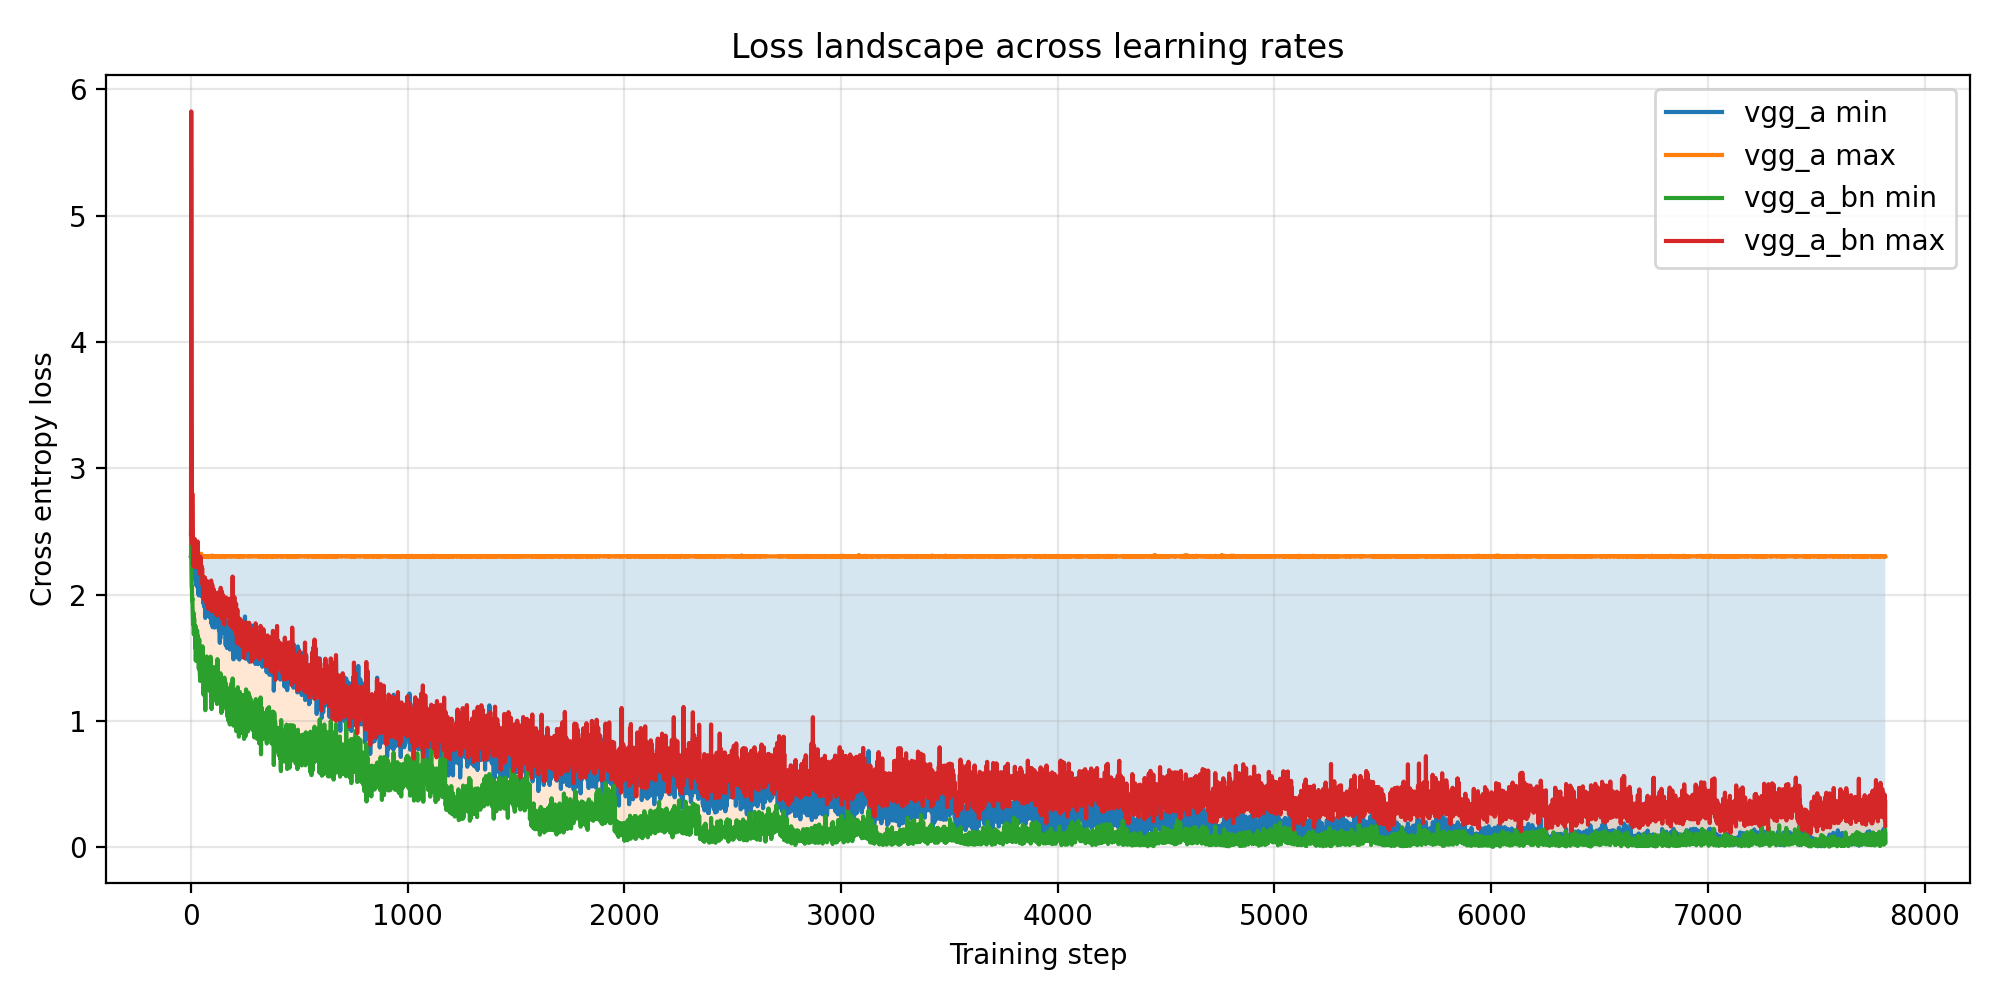
\includegraphics[width=0.95\linewidth]{figures/loss_landscape_comparison.png}
\caption{Loss landscape comparison for VGG-A and VGG-A-BN. The filled bands show
the loss variation across different learning rates at the same training step.}
\end{figure}

The loss landscape visualization shows that the BN model has a smoother and more
stable loss band across learning rates. The baseline VGG-A is much more
sensitive to the learning-rate choice, especially when the learning rate is too
large. This is consistent with the experimental result that VGG-A fails at
$2\times10^{-3}$, while VGG-A-BN remains trainable.

\section{Conclusion}

This project implemented CIFAR-10 classification models based on the provided
VGG-A code and extended it with Batch Normalization. The best result was obtained
by VGG-A-BN with learning rate $10^{-3}$, reaching 82.17\% validation accuracy
and 17.83\% error. Compared with VGG-A, Batch Normalization improves the best
accuracy and makes the model more stable under different learning rates.

The ablation experiments cover different filter widths, loss/regularization
settings, activation functions, and optimizers. The loss landscape visualization
further supports the interpretation that BN smooths the optimization behavior and
reduces sensitivity to learning-rate changes.

\appendix
\section{Reproducibility}

The main command used on the GPU server was:
\begin{verbatim}
nohup python run_pj2_gpu.py --epochs 20 --batch-size 128 \
  --num-workers 4 --device cuda:0 \
  --data-root codes/VGG_BatchNorm/data > train_full.log 2>&1 &
\end{verbatim}

The generated files used in this report are:
\begin{itemize}
    \item \texttt{pj2\_outputs/tables/summary.csv}
    \item \texttt{pj2\_outputs/tables/ablation\_summary.csv}
    \item \texttt{pj2\_outputs/figures/training\_curves.png}
    \item \texttt{pj2\_outputs/figures/loss\_landscape\_comparison.png}
    \item \texttt{pj2\_outputs/models/*.pt}
\end{itemize}

\end{document}
